\documentclass{endm}
\usepackage{endmmacro}
\usepackage{graphicx}

\usepackage{amssymb,amsmath,latexsym}
\usepackage[varg]{pxfonts}
%%%%%% ENTER ADDITIONAL PACKAGES
%\usepackage{graphics}
\usepackage{pst-all}
\usepackage{graphicx}
\usepackage{amsmath,amsfonts}
\usepackage{amssymb} % ADDED
\usepackage{times}
\usepackage{latexsym}
\usepackage{fancybox}
\usepackage{algorithm}
%\usepackage{algorithmic}
\usepackage{algorithmicx}
\usepackage{algpseudocode}
\usepackage{setspace}
\usepackage{courier}
\usepackage{verbatim}
\usepackage{hhline}
\usepackage{etex}
\usepackage{tikz}
\usetikzlibrary{calc,arrows,automata}
\usetikzlibrary{matrix,positioning,arrows,decorations.pathmorphing,shapes}
\usetikzlibrary{shapes,snakes}
\usepackage{graphicx}

\usepackage{mathrsfs}
\usepackage[a4paper, total={6in, 8in}]{geometry}
\usepackage{titlesec}
\newtheorem{prop_es}{Proposición}
%MACROS

\titlespacing{\subsection}
    {1pt}{1ex}{0ex}
%---------------
\usepackage{subfigure}
\usepackage{mathtools}
\usepackage{booktabs}
\usepackage{hyperref}

\tolerance=1
\emergencystretch=\maxdimen
\hyphenpenalty=10000
\hbadness=10000

\floatname{algorithm}{Algorithm}

\def\lastname{Toyos, Mangado, Piñeyro, Fasanello.}

\usepackage[english,spanish]{babel}

\begin{document}
% DO NOT REMOVE: Creates space for Elsevier logo, ScienceDirect logo% and ENDM logo
\begin{verbatim}
\end{verbatim}
\vspace{0.6 cm}
%Modifiqué el verbatim ese para que entrase el abstract en la cover...
\begin{frontmatter}

\title{Obligatorio 2 - Aplicaci\'on de Diferencias Finitas de la Ecuaci\'on de Calor
Unidimensional}

\subtitle{Grupo 36}

\author{Guillermo Daniel Toyos Marfurt,}
\author{Juan Jos\'e Mangado Esteves,}
\author{Martín Sebastián Piñeyro Olivera,}
\author{Ricardo Alejandro Fasanello Guillermo}

\address{Tutor: Juan Piccini}
\address{M\'etodos Num\'ericos 2020\\ Instituto de Matem\'atica y Estad\'istica\\ Facultad de Ingenier\'ia. Universidad de la Rep\'ublica\\ Montevideo, Uruguay}
\begin{abstract}
\setlength{\parindent}{12pt}
Se estudia el \textit{problema de Cauchy Dirichlet  para la ecuación del calor no homogénea} y con condición de borde nula en el caso unidimensional utilizando el método de integración $\theta$-método. Para ello se presenta una solución discreta al problema y se demuestra su correctitud de forma analítica junto a su implementación. Adicionalmente se encuentra un criterio de estabilidad asintótica para el caso particular donde $\theta=0$ y el sistema no tiene una fuente de generación calorífica. Lo cual asegura la convergencia del problema si la distancia finita entre cada instante del tiempo es menor el cuadrado de la diferencia entre cada punto del espacio sobre una constante. También se estudia experimentalmente el comportamiento del $\theta$-método para distintos valores de $\theta$ y se presentan representaciones gráficas de la evolución temporal de la temperatura a lo largo de la barra junto a su diferencia con el comando \textit{lsode} de \textit{Octave} observándose una mejor aproximación con $\theta=\frac{1}{2}$. El informe finaliza con un análisis del error del $\theta$-método en comparación con el comando \textit{lsode} mostrando que la solución presentada genera resultados similares a los de \textit{lsode} y su diferencia se puede reducir arbitrariamente reduciendo la distancia que se toma entre cada punto discreto del tiempo.
%Se estudia ,sobre un sistema unidimensional, la evoluci\'on del perfil de temperaturas $u(x,t)$ en funci\'on del
%tiempo. Para ello, dada una condici\'on inicial para el perfil de temperaturas y una fuente de generaci\'on
%calor\'ifica modelada por una funci\'on $f(x,t)$, se somete a pruebas el comando \textit{lsode} de
%\textit{Octave} junto con implementaciones de variantes del $\theta$-m\'etodo.Del mismo modo tambi\'en se pone a
%prueba dicho comando y m\'etodo cuando no est\'an inmersos en la fuente de generaci\'on calor\'ifica.
%El informe finaliza con la representaci\'on gr\'afica de los perfiles de temperaturas junto con la respectiva %evoluci\'on temporal de cada m\'etodo, y comparaciones de como evoluciona el error de los m\'etodos implementados %cuando se toma como referencia el comando \textit{lsode}.Se concluye que para $\theta = \frac{1}{2}$ , el %$\theta$-m\'etodo otorga una mejor aproximaci\'on que el resto de las variantes planteadas en lo que se refiere a %integrar respecto al tiempo el sistema de ecuaciones diferenciales.

\end{abstract}

\begin{keyword}
Ecuaciones diferenciales en derivadas parciales, Ecuación del calor, Métodos de integración, $\theta$-método
\end{keyword}

\end{frontmatter}
{
\hypersetup{linkcolor=black}
\tableofcontents
}
\section{Introducci\'on}\label{intro}
%La termodinámica es la rama de la física que estudia la conversión de la energía y el intercambio de la misma entre dos o más sistemas físicos, así como la capacidad de los sistemas para producir trabajo. El estudio de esta rama, del mismo modo que el estudio de sus leyes, tiene su importancia. Partiendo de nuestra vida cotidiana, por ejemplo, diversos electrodomésticos, como los microondas y las heladeras, son posibles gracias al trabajo de varios ingenieros que emplearon, entre otras cosas, la termodinámica. Incluso tiene su importancia a nivel industrial, ya que es algo imprescindible para definir propiedades y mezclas de diversas sustancias, procesando en base a esto la materia prima, y así elaborando diversos productos que a día de hoy la sociedad utiliza.\\

%En particular, se estudia un proceso llamado transferencia de calor, es decir, la propagación del calor en distintos medios. El calor se puede entender de dos maneras distintas, pero relacionadas. Por una parte, se define el calor como la energía que es intercambiada entre un cuerpo y un sistema, a raíz de la diferencia de temperatura entre los mismos (que, con el fin de buscar un equilibrio, un elemento va transfiriéndole energía al otro hasta llegar a la misma temperatura); mientras que por otra parte, se puede entender como un método en sí, para transferir energía.\\

%A modo de ejemplo, una cosa que sucede cotidianamente en nuestras vidas y de lo cual probablemente no nos percatamos, es el intercambio de energía en forma de calor que tienen los cuerpos y objetos con otros cuerpos.
%Por más que algo esté "caliente" o "frío", está constantemente realizando un intercambio de calor
%con todo a su alrededor.\\

%En este trabajo, vamos a estudiar cómo es y cómo calcular la ecuación del calor sobre una región, 
%y a lo largo de un transcurso del tiempo. Para poder adaptar un problema como este, donde se 
%hagan presentes dos o más variables independientes, se hace uso de las Ecuaciones diferenciales en 
%Derivadas Parciales, también conocidas como EDP. Entendiendo así, que la ecuación de calor es una del tipo de las %ya mencionadas.\\

Imagínese, lector, que usted se encuentra en un caluroso desierto y tiene una ardiente y fina barra de metal en sus manos. Ahora usted coloca en sus extremos dos cubos de hielo. ¿Que sucede? Este modelo físico puede modelarse mediante la siguiente ecuación en derivadas parciales conocida como la \textit{ecuación del calor no homogénea}:
\begin{equation*}
    \frac{\partial u}{\partial t}(x,t) -\mu \frac{\partial^2 u}{\partial x^2}(x,t) = f(x,t)
\end{equation*}
La variable $x$ representa la posición unidimensional en un segmento, $t$ el tiempo y $u(x,t)$ la temperatura de la barra en el punto $x$ e instante $t$. Supondremos que la barra es lo suficientemente fina y trataremos el problema en una dimensión, i.e. $x \in \mathbb{R}$. La función $f(x,t)$ modela una fuente de calor que calienta la barra uniformemente (el calor del desierto) y la constante $\mu$ es un coeficiente inherente al material. Como inicialmente la barra se encontraba caliente, tendremos una función $u_0(x)$ que modela la temperatura de la barra en el tiempo inicial del problema ($u(x,0)=u_0(x)$). Por último, los cubos de hielo en los extremos de la barra pueden modelarse como una condición que debe cumplir $u$: En ambos extremos de la barra, la temperatura es $0$ en todo instante. A este problema se lo conoce como \textit{problema de Cauchy Dirichlet para la ecuación del calor no homogénea con contorno de Dirichlet homogéneo}.\\
Si bien es posible resolver el problema mencionado analíticamente, en éste informe trataremos de hallar una aproximación de $u(x,t)$ utilizando una cierta familia de métodos de integración conocida como $\theta$-métodos. \\
El informe realiza los siguientes aportes:
\begin{itemize}
    \item Se construye paso a paso una aproximación a la ecuación del calor en diferencias finitas y un esquema de implementación.
    \item Demostración de distintas propiedades de la solución planteada: Orden de los errores, existencia de solución y caracterización del método planteado.
    \item Obtención de un criterio de estabilidad asintótica para el caso $\theta=0,f(x,t)=0$.
    \item Un estudio experimental con distintas simulaciones para confirmar la correctitud del algoritmo comparándolo con el comando \textit{“lsode”} de \textit{Octave}.
    \item Comparación del error de la solución propuesta con el comando \textit{“lsode”} para múltiples casos en una posición y tiempo dado.
\end{itemize}
El informe se organiza de la siguiente manera. La sección (\ref{AA}) trata sobre la metodología, planteo y análisis de la solución construida. La sección (\ref{Comparison}) presenta los resultados del análisis experimental. Finalmente, la sección (\ref{Conclusions}) presenta las conclusiones del trabajo.


\section{Problema a resolver}\label{Problem}
Dado un intervalo $[a,b]\subset\mathbb{R}$, una constante $\mu>0$, una función $u_0 : [a,b]\rightarrow\mathbb{R}$ y la función $u : [a,b]\times\mathbb{R}\rightarrow\mathbb{R}$ regida por la siguiente ecuación en derivadas parciales y condiciones iniciales:

\begin{equation*} \label{problema0}
    \begin{cases}
        u \in C^4 \ \text{en} \ (a,b)\times(0,+\infty) \  \text{y continua en} \  [a,b]\times[0,+\infty) \\
       \frac{\partial u}{\partial t}(x,t) -\mu \frac{\partial^2 u}{\partial x^2}(x,t) = f(x,t) \\
       u(x,0) = u_0(x), \ \forall x \in [a,b]\\
       u(a,t) = u(b,t) = 0, \ \forall t \in \mathbb{R}\\
    \end{cases}
\end{equation*}

Se desea hallar una aproximación de los valores de $u(x,t)$ en un espacio discretizado.
Es decir, transformando el problema infinitesimal en un problema de diferencias
finitas, hallar las soluciones de $u(x_j,t^k)$ para $x_j = a + jh$ con $j = \{1 \dots
N-1$\}, $h=\frac{(b-a)}{N}$ y $t^k=k\Delta t$, $k= \{1 \dots K\}$. Donde $N$ y $(\Delta t, K)$  definen la diferencia entre cada punto del espacio y tiempo respectivamente. 
\section{Metodolog\'ia}\label{AA}

\subsection{Estimador para \texorpdfstring{$\frac{\partial^2u}{\partial x^2}$}{du/dx} }
Dado un tiempo t fijo y suponiendo que $u$ es $C^{4}$ según la variable espacial, se puede escribir el desarrollo de Taylor de $u$ en $(\bar{x},t)$ como: 
\begin{equation} \label{p1taylor1}
   u(\bar{x}+h,t) = u(\bar{x},t) + h\frac{\partial u}{\partial x}(\bar{x},t) +
   \frac{h^2}{2!}\frac{\partial^{2} u}{\partial x^2}(\bar{x},t) +
   \frac{h^3}{3!}\frac{\partial^3u}{\partial x^{3}}(\bar{x},t) + R_3(\theta,t)
\end{equation} 
Donde $R_3$ es el resto de Lagrange de orden 4 \cite[p. 348]{apostol}
\begin{equation*}
R_3(\theta,t) = \frac{h^4}{4!}\frac{\partial^4u}{\partial x^4}(\theta,t), \ \ \theta \in [\bar{x}, \bar{x}+h]
\end{equation*}
Realizando el cambio de variable $h \coloneqq -h$ en (\ref{p1taylor1}) se obtiene: 
\begin{equation} \label{p1taylor2} 
   u(\bar{x}-h,t) = u(\bar{x},t) - h\frac{\partial u}{\partial x}(\bar{x},t) +
   \frac{h^2}{2!}\frac{\partial^2 u}{\partial x^2}(\bar{x},t)
   -\frac{h^3}{3!}\frac{\partial^3u}{\partial x^3}(\bar{x},t) + R_4(\theta^*,t), \\
   \theta^* \in [\bar{x}-h, \bar{x}]
\end{equation} 
Sumando (\ref{p1taylor1}) y (\ref{p1taylor2}) se obtiene:
\begin{align*}
 \underbrace{\frac{u(\bar{x}+h,t) + u(\bar{x}-h,t) -2u(\bar{x},t)}{h^2}}_{\text{Estimador de $\frac{\partial^2 u}{\partial x^2}$}} = \frac{\partial^2u}{\partial x^2}+\underbrace{h^2\bigg[\frac{1}{4!}\frac{\partial^4u}{\partial x^4}(\theta,t) +\frac{1}{4!}\frac{\partial^4u}{\partial x^4}(\theta^*,t)\bigg]}_{\text{Error $E_T$}}
\end{align*}

Para h suficientemente pequeño, se puede suponer que $\theta = \theta^* = \bar{x}$. Así el error de la aproximación $E_T = h^2\frac{2}{4!}\frac{\partial^4}{\partial x^4}(\bar{x},t)$.  Por lo que la aproximación es de segundo orden con respecto a h. \\

Utilizando este estimador se puede \textit{semidiscretizar} el problema. i.e. $u$ se aproxima en $N$ puntos a distancia $h$ cada uno. Dejando la aproximación de $u$ en función solamente del tiempo: (Denotamos $u_j: \mathbb{R} \rightarrow \mathbb{R} \ / u_j(t)=u(x_j,t)$ ) 
\begin{equation} \label{sistema_jj}
\begin{cases} 
   \frac{d u_j}{d t}(t) - \frac{\mu}{h^2}(u_{j-1}(t) -2u_j(t) + u_{j+1}(t)) = f_j(t),  \ \ j \in \{1 \dots N-1\}\\
   u_0(t) = u_N(t) = 0
\end{cases}
\end{equation}
Este sistema se puede escribir matricialmente mediante los siguientes vectores y matrices:
\begin{equation*}
    \boldsymbol{u}(t)=
        \begin{pmatrix}
            u_1(t)\\
            \vdots\\
            u_{N-1}(t)\\
    \end{pmatrix}
    \quad
    \boldsymbol{f}(t)=
        \begin{pmatrix}
            f_1(t)\\
            \vdots\\
            f_{N-1}(t)\\             
        \end{pmatrix}
    \qquad
    \boldsymbol{u_0}=
        \begin{pmatrix}
        u_{0}(x_{1})\\
        \vdots\\
        u_{0}(x_{N-1})\\             
        \end{pmatrix}
    \qquad
    \boldsymbol{A}= 
        \begin{pmatrix}
        2 & -1 & 0 & \dots & 0 \\
        -1 & 2 & -1 & \dots & 0 \\
        \vdots & &\ddots & & \vdots \\
        0 & \dots & -1 & 2 & -1 \\
        0 & \dots & 0 & -1 & 2 \\
        \end{pmatrix}
\end{equation*}
Específicamente, la matriz $\boldsymbol{A} \in \mathcal{M}^{(N-1)\times(N-1)}$ es una matriz tri-diagonal de Topelitz \cite{topelitz} cuyas entradas no nulas son: 
\begin{align} \label{Arules}
 a_{i,i} = 2 \\
 a_{i+1,i} = -1  &&   \forall i \in \bigg\{ 1, \dots, N - 1\bigg\} \\
 a_{i,i+1} = -1
\end{align}

Como $u_0(t)=u_N(t)=0$. El sistema \ref{sistema_jj} es equivalente a:
\begin{equation} \label{sistema_Adt}
\begin{cases} 
   \frac{d \boldsymbol{u}}{d t}(t) = -\frac{\mu}{h^2} \boldsymbol{A} \boldsymbol{u}(t) + \boldsymbol{f}(t) \\
   \boldsymbol{u}(0) = \boldsymbol{u_0}
\end{cases}
\end{equation}

%--------- Ejercicio 3 --------------

\subsection{Autovalores y autovectores de la matriz A}

A continuación se procede a estudiar el espectro de la matriz $\boldsymbol{A}$. Lo cual será útil para probar la correctitud de los métodos de resolución del sistema que se presentarán más adelante.
\begin{prop_es} \label{VAPyVEP}
Los valores propios $\lambda_{j}$, y los vectores propios $q_{j}$, $j \in \{1\dots N-1\}$,  de $\boldsymbol{A}$ son de la forma:

\begin{align*}
    & \lambda_{j} = 2 \bigg(1 - \cos{\bigg(j\frac{\pi}{N}\bigg)} \bigg) \\
    & q_{j} = \bigg(\sin{\bigg(j\frac{\pi}{N}\bigg)} ,\sin{\bigg(2j\frac{\pi}{N}\bigg)} ,\dots,\sin{\bigg((N-1)j\frac{\pi}{N} \bigg)} \bigg)^{T}
\end{align*}
\end{prop_es}
\begin{proof}
Basta con verificar que $\lambda_{j}$ y $q_j$ cumplen la definici\'on de valores y vectores propios:

\begin{equation*}
    (\forall j \in \{1,\dots,N-1\})(A\cdot{q_{j}} = \lambda_{j}\cdot{q_{j}} )
\end{equation*}

Tomando un $j$ genérico:
\begin{equation*}
    \lambda_{j}q_{j} = 2 \bigg(1 - \cos{\bigg(j\frac{\pi}{N}\bigg)} \bigg) \cdot
    \begin{pmatrix}
        \sin{\bigg(j\frac{\pi}{N}\bigg)}\\
        \sin{\bigg(2j\frac{\pi}{N}\bigg)}\\
        \vdots\\
        \sin{\bigg((N-1)j\frac{\pi}{N}\bigg)}\\
    \end{pmatrix}\
    = \begin{pmatrix}
        2\sin{\bigg(j\frac{\pi}{N}\bigg)} - 2\cos{\bigg(j\frac{\pi}{N}\bigg)}\sin{\bigg(j\frac{\pi}{N}\bigg)}\\
        2\sin{\bigg(2j\frac{\pi}{N}\bigg)} - 2\cos{\bigg(j\frac{\pi}{N}\bigg)}\sin{\bigg(2j\frac{\pi}{N}\bigg)}\\
        \vdots\\
        2\sin{\bigg((N-1)j\frac{\pi}{N}\bigg)} - 2\cos{\bigg(j\frac{\pi}{N}\bigg)}\sin{\bigg((N-1)j\frac{\pi}{N}\bigg)}\\
    \end{pmatrix}
\end{equation*}

Sea $k$ una entrada cualquiera del vector $\lambda_{j}q_{j}$, y usando la identidad
trigonom\'etrica $2\cos{(b)}\sin{(a)} = \sin{(a+b)} + \sin{(a-b)}$, se tiene que: 

\begin{equation*}
    (\lambda_{j}q_{j})_{k} = 2\sin{\bigg(kj\frac{\pi}{N}\bigg)} - \bigg(\sin{\bigg((k+1)j\frac{\pi}{N}\bigg)} + \sin{\bigg((k-1)j\frac{\pi}{N}\bigg)} \bigg) 
    \ , \forall \ j,k \in \{1,\dots,N-1\}
\end{equation*}

Por otro lado:
\begin{equation*}
    A\cdot{q_{j}} = \begin{pmatrix}
        2 & -1 & 0 & \dots & 0 \\
        -1 & 2 & -1 & \dots & 0 \\
        \vdots & &\ddots & & \vdots \\
        0 & \dots & -1 & 2 & -1 \\
        0 & \dots & 0 & -1 & 2 \\
    \end{pmatrix}
    \cdot 
    \begin{pmatrix}
         \sin{\bigg(j\frac{\pi}{N}\bigg)}\\
        \sin{\bigg(2j\frac{\pi}{N}\bigg)}\\
        \vdots\\
        \sin{\bigg((N-1)j\frac{\pi}{N}\bigg)}\\
    \end{pmatrix}
\end{equation*}

Para $k \in \{ 2,\dots, N-2 \}$ se cumple que: 
\begin{equation*}
    (A\cdot q_{j})_{k} = 2\sin{\bigg(kj\frac{\pi}{N}\bigg)} -
    \bigg(\sin{\bigg((k+1)j\frac{\pi}{N}\bigg)} + \sin{\bigg((k-1)j\frac{\pi}{N}\bigg)}
    \bigg) 
\end{equation*}

Resta ver los casos $k = 1$ y $k = N-1$ : 

\begin{equation*}
   \begin{rcases}
    & (A\cdot q_{j})_{1}  = 2 \sin{\bigg(j\frac{\pi}{N}\bigg)} -
    \sin{\bigg(2j\frac{\pi}{N}\bigg)} \\
    & (\lambda_{j}\cdot q_{j})_{1} = 2 \sin{\bigg(j\frac{\pi}{N}\bigg)} - 
    \bigg( \sin{\bigg(2j\frac{\pi}{N}\bigg)} + \sin{\bigg((1-1)j\frac{\pi}{N}\bigg)}
    \bigg)
   \end{rcases} \underset{\sin(0) = 0}{\Longrightarrow} (A\cdot q_{j})_{1} = (\lambda_{j}\cdot q_{j})_{1} 
\end{equation*}

\begin{equation*}
   \begin{rcases}
    & (A\cdot q_{j})_{N-1}  = 2 \sin{\bigg((N-1)j\frac{\pi}{N}\bigg)} -
    \sin{\bigg((N-2)j\frac{\pi}{N}\bigg)} \\
    & (\lambda_{i}\cdot q_{j})_{N-1} = 2 \sin{\bigg((N-1)j\frac{\pi}{N}\bigg)} - 
    \bigg( \sin{\bigg(\frac{N}{N}j \pi \bigg)} + \sin{\bigg((N-2)j\frac{\pi}{N}\bigg)}
    \bigg)
   \end{rcases} \underset{j\in \mathbb{N} \rightarrow \sin(j\pi)=0 }{\Longrightarrow}
   (A\cdot q_{j})_{N-1} = (\lambda_{j}\cdot q_{j})_{N-1} 
\end{equation*}

Se concluye que:\quad $ A\cdot q_{j} = \lambda_{j}\cdot q_{j},\quad \forall j \in \{1,\dots, N-1\} $. \end{proof}
%--------- end Ejercicio 3 ----------


%------- Ejercicio 4 -------
\subsection{\texorpdfstring{$\theta$-m\'etodo}{Theta-metodo}}

El $\theta$-m\'etodo es un esquema de integraci\'on, el cual se basa en aproximar una funci\'on mediante una combinaci\'on conexa de las pendientes en dos puntos discretos. La forma general del $\theta$-m\'etodo, para el problema $\frac{dy}{dt}=f(t,y), y(x_0)=t_0$, es la siguiente \cite[p.36]{slidetheta}:
\begin{equation} \label{thetageneral}
    y_{n+1} = y_n + h\bigg[ (1-\theta)f(t_n,y_n)+\theta f(t_{n+1},y_{n+1})\bigg], \ \ \theta \in [0,1]
\end{equation}

La idea del mismo se ilustra en el diagrama de la Figura \ref{fig:Diagrama}. La cual muestra que el parámetro $\theta$ es el que define la cantidad de área azul que se va a tomar para calcular el área debajo de la curva en el intervalo $[x_j,x_{j+1}]$. Este hecho muestra que el $\theta$-m\'etodo es una generalización de varios métodos de integración:
\begin{itemize}
    \item $\theta=0$: “Método de Euler hacia adelante”
    \item $\theta=\frac{1}{2}$: “Método del trapecio”
    \item $\theta=1$: “Método de Euler hacia atrás”
\end{itemize}
Comprobemos el caso particular donde $\theta=\frac{1}{2}$. En forma general, el Método del Trapecio se define como \cite[p.111]{notasteo}:
\begin{equation*}
    y_{n+1}=y_n+\frac{h}{2}\bigg[f(t_n,y_n)+f(t_{n+1},y_{n+1})\bigg]
\end{equation*}
Es claro que cuando $\theta=\frac{1}{2}$, la expresión anterior coincide con \ref{thetageneral}.
\begin{figure}[htp]
    \centering
    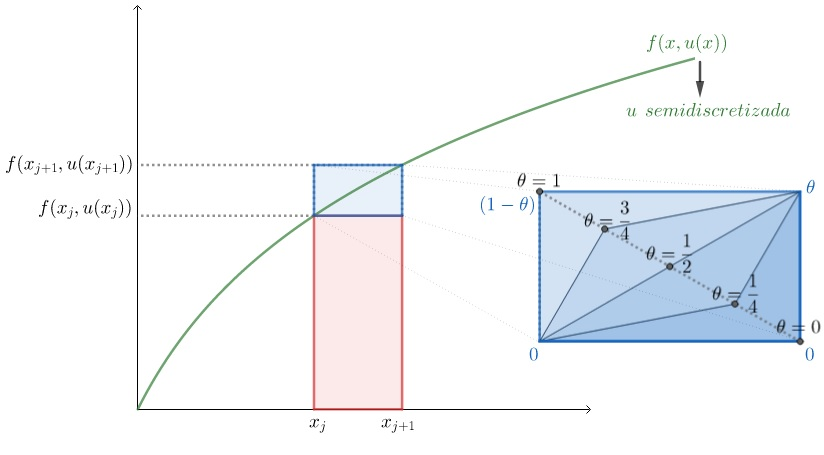
\includegraphics[width=15cm]{Diagrama}
    \caption{Ilustración del $\theta$-m\'etodo. Notar que en la imagen $f(x,t)=\frac{-\mu}{h^2}A\cdot u(t)+f^*(x,t)$, donde $f^*$ es la función de generación calorífica del sistema.}
    \label{fig:Diagrama}
\end{figure}

Discretizando ahora el tiempo, sea $\Delta t > 0$ un paso del tiempo constante, se denotan los vectores como $\textbf{v}^{k}$ para referirse a los mismos evaluados en un tiempo $t^{k} = k \Delta t$. El siguiente sistema resulta de la aplicaci\'on del $\theta$-m\'etodo para la ecuaci\'on \ref{sistema_Adt}:

\begin{equation} \label{NEOTHETA}
    \begin{cases}
        \frac{\textbf{u}^{k+1} - \textbf{u}^{k}}{\Delta t} = - \frac{\mu}{h^2} \textbf{A}(\theta \textbf{u}^{k+1} + (1 - \theta)\textbf{u}^k) + \theta \textbf{f}^{k+1} + (1-\theta)\textbf{f}^k, k = 0, 1, ..., K\\
        \textbf{u}^0 = \textbf{u}_0
    \end{cases}
\end{equation}
Expresando dicho sistema en notaci\'on matricial:
\begin{equation} \label{FINALSYS}
    \begin{cases}
        \textbf{D u}^{k+1} = (I - \frac{\mu}{h^2} \Delta t (1-\theta) \textbf{A})\textbf{u}^k + \textbf{g}^{k+1}\\
        \textbf{u}^0 = \textbf{u}_0
    \end{cases}
\end{equation}\\

donde $\textbf{g}^{k+1} = \Delta t (\theta \textbf{f}^{k+1} + (1-\theta)\textbf{f}^{k})$, y $\textbf{D} = (I + \frac{\mu}{h^2} \theta \Delta t \textbf{A})$\\

Observar que el problema de aproximar la soluci\'on de una ecuaci\'on en derivadas parciales se transform\'o en resolver una recurrencia de sistemas lineales. Para poder resolver los mismos, es necesario que la matriz D sea invertible.\\

\begin{prop_es}\label{dinver}
    La matriz $\textbf{D}$ es invertible.
\end{prop_es}
\begin{proof}
Para probar que la matriz $\textbf{D}$ es invertible, se usar\'an las siguientes propiedades y equivalencias: 
\begin{enumerate}
    \item $\textbf{D}$ es invertible $\Leftrightarrow det(\textbf{D}) \neq 0 \Leftrightarrow \lvert \lambda \rvert > 0 \ \ \forall \lambda$ autovalor de  $\textbf{D}$%Citar?
    \item $\lambda$ es vap de $\textbf{A} \Rightarrow \alpha\lambda$ es vap de $\alpha\textbf{A}$
\end{enumerate}

Por definici\'on, $\lambda$ es autovalor de $\textbf{D} \Leftrightarrow det(\textbf{D} - \lambda I) = 0$
\begin{gather*}
\Leftrightarrow det(I + \frac{\mu}{h^2}\theta \Delta t \textbf{A} - \lambda I) = 0 \\
\Leftrightarrow \\
det(\frac{\mu}{h^2}\theta \Delta t \textbf{A} - (\lambda - 1)I) = 0\\
%Haciendo un cambio de variable: $\lambda^{*} = \lambda - 1$: 
\overset{\lambda^{*} = \lambda - 1}{\iff}\\
det(\frac{\mu}{h^2}\theta \Delta t \textbf{A} - (\lambda^{*})I) = 0\\
\end{gather*}

Observar que estos son, por definici\'on, los autovalores de la matriz $\frac{\mu}{h^2}\theta\Delta t \textbf{A}$. Utilizando \textit{(ii)} y dado el hecho que se conocen los autovalores de $\textbf{A}$ (Prop \ref{VAPyVEP}): 
\begin{gather*}
\lambda^{*} = \frac{\mu}{h^2}\theta\Delta t 2(1-\cos(j \frac{\pi}{N}))\\
\overset{\lambda^{*} = \lambda - 1}{\iff}\\
\lambda = \frac{\mu}{h^2}\theta\Delta t 2(1-\cos(j \frac{\pi}{N}))+1 \\
\end{gather*}
Como $\mu, h^2, \theta, \Delta t$ son positivos ($>0$) y $(1-\cos(j\frac{\pi}{N})) \in (0, 2) \ \ \forall j \in \{1 \dots N-1\}$, tenemos que $\lambda \ge 1 \Rightarrow |\lambda | > 0 \ \forall \lambda$ autovalor de  $\textbf{D} \overset{(i)}{\Leftrightarrow} \textbf{D}$ es invertible.
\end{proof}
%------- end Ejercicio 4 -------
\subsection{\texorpdfstring{Caso $\theta=0, \boldsymbol{f}=0$}{Theta 0 f 0}} \label{casolindo}

Para este caso particular, donde $\boldsymbol{f}^k = 0 \ \ \forall k$.
Se tiene a partir de la ecuación \ref{FINALSYS} la siguiente recurrencia:
\begin{equation} \label{theta00}
     \boldsymbol{u}^k = \boldsymbol{E}^k\boldsymbol{u}^0 \ \ \text{con} \ \ k=\{1\dots K\} \ \ \text{y} \ \ E =(I-\frac{\mu}{h^2}\Delta tA)
\end{equation}
Donde $\boldsymbol{E}^k$ es la $k$-ésima potencia de $\boldsymbol{E}$ y $\boldsymbol{u}^0=\boldsymbol{u_0}$.\\

Para demostrar la estabilidad de este método, se prueba la siguiente proposición:
\begin{prop_es} \label{dem6}
    $\rho(\boldsymbol{E}) < 1 \iff \Delta t < \frac{h^2}{2\mu}$, donde $\rho$ es el radio espectral.
\end{prop_es}

\begin{proof}
Para poder realizar la demostración, será de utilidad la siguiente propiedad:
\begin{enumerate} \label{sumvaps}
    \item Sean $A,I \in \mathcal{M}^{n \times n}$, donde $A$ es una matriz diagonalizable cualquiera e $I$ la identidad.
    Sean $\lambda_{1},\dots ,\lambda_{n}$ los autovalores de $A$, %y sean $v_{1},\dots,v_{n}$ sus respectivos
    %autovectores.\\
    entonces $A+I$ tiene %autovectores $v_{1},\dots,v_{n}$, y sus respectivos 
    autovalores de la forma $\lambda_{1} +
    1,\dots ,\lambda_{n} + 1$ 
\end{enumerate}
    

Sea $\lambda$ un vap de A, y $\lambda^*$ un vap de E genérico. Por la propiedad mencionada anteriormente y (ii) de la proposici\'on \ref{dinver} , tenemos que:
\begin{gather*}
    \lambda^* = 1´+ \frac{-\mu}{h^2}\Delta t\lambda \overset{\text{Prop \ref{VAPyVEP}}}{\iff} \lambda^*_j = 1- \frac{\mu}{h^2}\Delta t2(1-cos(j\frac{\pi}{N}))\\
    \Rightarrow \\ 
    p(E) < 1 \iff \Bigg|1 - \frac{2\mu}{h^2}\Delta t \big(1-cos(j\frac{\pi}{N})\big) \Bigg| < 1 \ \ \forall j
\end{gather*}
Tomando un $j$ genérico:
\begin{equation*}
    -2 < -\frac{\mu}{h^2}\Delta t2(1-cos(j\frac{\pi}{N}) < 0
\end{equation*}
Por un lado:
\begin{equation}
     -\frac{\mu}{h^2}\Delta t2(1-cos(j\frac{\pi}{N}) < 0 \iff -\frac{\mu}{h^2}\Delta t < 0.
\end{equation}
  Lo cual es cierto. Pues el término $(1- cos(j\frac{\pi}{N})) \in (0,2)$, por lo que no afecta al signo de la expresión y $\mu,h,\Delta t$ son positivos.\\
Por el otro:
\begin{equation*}
  -2 < -\frac{\mu}{h^2}\Delta t2(1-cos(j\frac{\pi}{N})) \iff
  \frac{\mu}{h^2} \Delta t\big(1-cos(j\frac{\pi}{N})\big) < 1 \overset{N \coloneqq \frac{b-a}{h}}{\iff}
  \frac{\mu}{h^2}\Delta t\big(1-cos(\frac{j\pi h}{b-a})\big) < 1
\end{equation*}
Entonces basta probar que:
\begin{equation}
    \frac{\mu}{h^2}\Delta t\big(1-cos(\frac{j\pi h}{b-a})\big) < 1 \iff \Delta t < \frac{h^2}{2\mu}
\end{equation}
$(\Rightarrow)$ Suponiendo que $\frac{\mu}{h^2}\Delta t\big(1-cos(\frac{j\pi h}{b-a})\big) < 1$:
\begin{equation}
    \frac{\mu}{h^2}\Delta t\big(1-cos(\frac{j\pi h}{b-a})\big) < 1 \Rightarrow
    \Delta t < \frac{h^2}{\mu}\cdot\frac{1}{\big(1-cos(\frac{j\pi h}{b-a})\big)} \overset{(*)}{\Rightarrow}
    \Delta t < \frac{h^2}{2\mu}
\end{equation}
$(*)$ Como $\inf_{j \in \{1\dots N-1\}}  \Bigg\{\frac{1}{\big(1-cos(\frac{j\pi h}{b-a})\big)}\Bigg\} = \frac{1}{2}$, se cumple particularmente que $\Delta t < \frac{h^2}{2\mu}$. \\
$(\Leftarrow)$ Suponiendo por hipótesis que $\Delta t < \frac{h^2}{2\mu}$:
\begin{equation}
    \frac{\mu}{h^2}\Delta t\big(1-cos(\frac{j\pi h}{b-a})\big) \overset{(H)}{<}
    \frac{1}{2}\big(1-cos(\frac{j\pi h}{b-a})\big) \overset{(**)}{<} 1
    \Rightarrow
    \frac{\mu}{h^2}\Delta t\big(1-cos(\frac{j\pi h}{b-a})\big) < 1
\end{equation}
$(**)$ Como la expresión $\big(1-cos(\frac{j\pi h}{b-a})\big)$ está acotada entre $(0,1)$ se cumple particularmente que $\big(1-cos(\frac{j\pi h}{b-a})\big) < 1$. \end{proof}
Utilizaremos la proposición anterior para demostrar que sí $\Delta t < \frac{h^2}{2\mu}$, el sistema es asintóticamente estable.
\begin{prop_es} \label{asintprop}
\begin{equation*}
    \Delta t < \frac{h^2}{2\mu} \Rightarrow \lim_{k\to\infty} \boldsymbol{u}^k = \boldsymbol{0}
\end{equation*}
\end{prop_es}
\begin{proof}
Recordando la siguiente propiedad del \'algebra lineal: $\boldsymbol{E}v = \lambda v \Rightarrow \boldsymbol{E}^k v = \lambda^k v$. \\
Dado que todos los vaps de $\boldsymbol{E}$ son distintos entre sí (Prop \ref{VAPyVEP}), E es diagonalizable. i.e $\exists P \in \mathcal{M}^{(N-1)\times(N-1)} / \boldsymbol{E} = P\boldsymbol{D}P^{-1}$.

Por prop \ref{dem6}, tenemos que $\rho(E) < 1 \Rightarrow |\lambda_j| < 1 \ \ \forall j \in \{1\dots N-1\} \Rightarrow lim_{k\to\infty} \boldsymbol{D}^k = \boldsymbol{0} $.
Como $\boldsymbol{E}^k = P\boldsymbol{D}P^{-1}P\boldsymbol{D}P^{-1}\dots = P\boldsymbol{D}^kP^{-1} \Rightarrow lim_{k\to\infty} \boldsymbol{E}^k = lim_{k\to\infty} P\boldsymbol{D}^kP^{-1} = \boldsymbol{0} $.\\
Entonces $lim_{k\to\infty} \boldsymbol{u}^k = lim_{k\to\infty} \boldsymbol{E}^ku^0 = \boldsymbol{0}$
\end{proof}
%------ Ejercicio 7 初めーーーーー
\subsection{Error analítico del \texorpdfstring{$\theta$-método}{Theta-metodo}} \label{Errortheta}

Se procede a estudiar analíticamente el error del $\theta$-método respecto al paso del tiempo $\Delta t$ con $x$ y $t$ fijos.

Despejando $u^{k+1}$ de la ecuación \ref{NEOTHETA}
\begin{equation}
    u^{k+1} = u^k - \Delta t\Bigg( (1-\theta)\underbrace{(-\frac{\mu}{h^2} A u^k + f^k)}_{\text{$=\frac{du^k}{dt}$ (\ref{sistema_Adt})}} + \theta \underbrace{(-\frac{\mu}{h^2} A u^{k+1}+f^{k+1})}_{\text{$=\frac{du^{k+1}}{dt}$ (\ref{sistema_Adt})}}\Bigg)
\end{equation}
Igualando la expresión anterior a su desarrollo de Taylor para $u^{k+1}$ y reemplazando $\frac{du^{k+1}}{dt}$ también por su respectivo desarrollo de Taylor se tiene que:
\begin{multline*}
    u^k+\Delta t \frac{du^k}{dt}+\frac{1}{2}\Delta t^2 \frac{d^2 u^k}{dt^2}+\frac{1}{6}\Delta t^3 \frac{d^3 u^k}{dt^3} + \frac{1}{4!}\Delta t^4 \frac{d^4 u(\theta)}{dt^4} = \\
    u^k+\Delta t (1-\theta) \frac{dt u^k}{dt}+ \Delta t \theta ( \frac{dt u^k}{dt}+ \Delta t \frac{d^2 u^k}{dt^2}+ \frac{1}{2} \Delta t^2 \theta \frac{d^3 u^k}{dt^3} + \frac{1}{6} \Delta t^3 \frac{d^4 u(\bar{\theta})}{dt^4}\\
    \theta,\bar{\theta} \in [t^k,t^{k+1}]
\end{multline*}
Desarrollando la ecuación se obtiene la siguiente expresión para el error de truncamiento:
\begin{equation}
    E_T = (\theta - \frac{1}{2})\Delta t^2 \frac{d^2 u^k}{dt^2}+ (\frac{1}{6}-\frac{\theta}{2})\Delta t^3 \frac{d^3 u^k}{dt^3}+\frac{1}{4!}\Delta t^4 \frac{d^4 u(\theta^*}{dt^4} +  \frac{1}{6}\Delta t^4 \frac{d^4 u(\bar{\theta})}{dt^4}
\end{equation}
Observar que sí $\theta = \frac{1}{2}$ el termino $\Delta t^2$ desaparece. Por lo tanto, el orden del error del  $\theta$-método respecto a $\Delta t$ es $2$ sí $\theta = \frac{1}{2}$ y $1$ sí $\theta \neq \frac{1}{2}$. Es decir, el error del método será de orden 2 cuando el mismo es equivalente al método del trapecio. 
\subsection{Implementación}
En esta última subsección se muestra una implementación del $\theta$-método, utilizando el esquema \ref{FINALSYS}, en pseudocódigo (Algo \ref{thetalggeneral}). Se pasan como parámetros $\theta, N, \Delta t, K$. Y se retorna una matriz $ M \in \mathcal{M}^{(N+1)\times(K+1)}$ donde $M_{i,j}=u(x_i,t^j) : x_i=a+i.h$ y $t^j = j.\Delta t$ donde $u$ es la aproximación de la solución provista por el método. Adicionalmente se pasan los parámetros $a, b, u_0, f, \mu$ que describen al problema.
\begin{algorithm}[H]
\caption{$\theta$-método}
\label{thetalggeneral}
\small
\centering
\begin{algorithmic}[1] 
\Require $\theta$ N $\Delta t$ K a b $\mu \ f \ u_0$ \Comment{$\theta \in [0,1], \ b>a, \ f:\mathbb{R}\times\mathbb{R}\rightarrow\mathbb{R}, \ u_0:\mathbb{R}\rightarrow\mathbb{R}$}
    \State{$h \leftarrow \frac{b-a}{N} $}
    \State{$A \leftarrow \{\mathcal{M}^{(N-1)\times(N-1)} : $ cumple las reglas \ref{Arules}$\}$}
    \State{$D \leftarrow I_{N-1} + \frac{mu}{h^2}.\theta.\Delta t \cdot A$ \Comment{$I$ matriz identidad}}
    \State{$F \in \mathcal{M}^{(N+1)\times(K+1)}$}
    \For{$n = 1:N+1 $}
        \For{$k = 0:K $}
            \State{$F(n,k+1) \leftarrow f(a+n.h,\Delta t.k)$}
        \EndFor
    \EndFor
    \State{$g \in \mathcal{M}^{(N+1)\times(K+1)}$}
    \For{$n = 1:N+1 $}
        \For{$k = 1:K $}
            \State{$g(n,k) \leftarrow \Delta t\Bigg(\theta.F\Big(a+h.n,(k+1)\Big).\Delta t)+(1-\theta)F\Big(a+h.n,k.\Delta t\Big)\Bigg)$}
        \EndFor
    \EndFor
    \State{$M \in \mathcal{M}^{(N+1)\times(K+1)} : M=\boldsymbol{0}^{(N+1)\times(K+1)}$}
    \For{$n=1:N$}
        \State{$M(a+h.n,1) \leftarrow u_0(a+h.n)$}
    \EndFor
    \State{$b \in \mathcal{M}^{(N-1)\times1}$}
    \For{$k=2:K+1$}
        \State{$b \leftarrow \Bigg(I_{N-1} - \frac{\mu}{h^2}\Delta t(1-\theta)A\Bigg)\cdot M(2:N,k-1)+g(2:N,k)$}
        \State{$M(2:N,k) \leftarrow x : D\cdot x = b$}
    \EndFor\\
\Return $M$ 
\end{algorithmic}
\end{algorithm}
Para el caso particular \ref{casolindo} es posible implementar un algoritmo más simple mediante el esquema \ref{theta00} (Algo \ref{thetalg0}). En este algoritmo se toman como parámetros $N, \Delta t, K$ más $u_0, \ a, \ b, \ \mu$ relacionados con el problema:
\begin{algorithm}[H] 
\caption{$\theta$-método en el caso $\theta=0, f(x,t)=0 \forall x,t$}
\label{thetalg0}
\small
\centering
\begin{algorithmic}[2]
\Require N $\Delta t$ K a b $\mu \ u_0$ \Comment{$b>a,\ u_0:\mathbb{R}\rightarrow\mathbb{R}$}
    \State{$h \leftarrow \frac{b-a}{N} $}
    \State{$A \leftarrow \{\mathcal{M}^{(N-1)\times(N-1)} : $ cumple las reglas \ref{Arules}$\}$}
    \State{$M \in \mathcal{M}^{(N+1)\times(K+1)} : M=\boldsymbol{0}^{(N+1)\times(K+1)}$}
    \For{$n=1:N$}
        \State{$M(a+h.n,1) \leftarrow u_0(a+h.n)$}
    \EndFor
    \State{$E \leftarrow I_{N-1} - \frac{\mu}{h^2 \Delta t}\cdot A$}
    \State{$M \in \mathcal{M}^{(N+1)\times(K+1)} : M=\boldsymbol{0}^{(N+1)\times(K+1)}$}
    \For{$k=2:K+1$}
        \State{$M(2:N,k) \leftarrow E^k \cdot M(2:N,1)$}
    \EndFor\\
\Return $M$ 
\end{algorithmic}
\end{algorithm}
\section{An\'alisis Experimental}\label{Comparison}

Para el análisis experimental se realizó una implementación del theta método en \textit{Octave}. La simulación consta de una barra de longitud 1 ($[a,b]=[0,1]$) con coeficiente de conductividad térmica $\mu=1$. Una función $u_0(x)=1000x(1-x)(1+\frac{3}{2}x^3)$ que define la temperatura en $t^0$. Y una función $f(x,t)$ que representa una fuente de generación calorífica. 
Para la comparación de resultados resolveremos también el problema utilizando la función \textit{lsode} de \textit{Octave}, la cual es un solucionador de ecuaciones diferenciales ordinarias. \cite{lsode}

\subsection{Simulación del \texorpdfstring{$\theta$-método}{Theta-metodo} con \texorpdfstring{$f(x,t)=1000\sqrt{|1-t|}$}{función generación externa}} \label{simusqrt}
Para este caso particular, el sistema de ecuaciones diferenciales \ref{FINALSYS} resulta:
\begin{equation}
    \frac{d\boldsymbol{u}}{dt}(t) = -\frac{1}{h^2}\boldsymbol{A}.\boldsymbol{u(t)}+
    \begin{pmatrix}
        1000.\sqrt{|1-t|}\\
        \vdots\\
        1000.\sqrt{|1-t|}\\
    \end{pmatrix}\
\end{equation}
Podemos representar la barra como un segmento al cual cada punto del mismo le corresponde una temperatura.
Para el problema presentado, el perfil de temperaturas en $t=0$ puede representarse de la siguiente manera (La referencia de los colores se encuentra en la figura \ref{fig:lsodesnip}):
\begin{center}
    \begin{figure}[H]
        \centering
        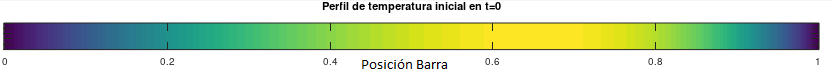
\includegraphics[scale=0.6]{hetmap_temp0.PNG}
        \caption{}
        \label{fig:barra0}
    \end{figure}
\end{center}
Utilizando el comando \textit{lsode} de Octave, podemos realizar una simulación de la evolución de la temperatura de la barra en el tiempo. La misma se puede visualizar tanto como un \textit{heatmap} o como una gráfica tridimensional:
\begin{figure}[H]
    \centering
    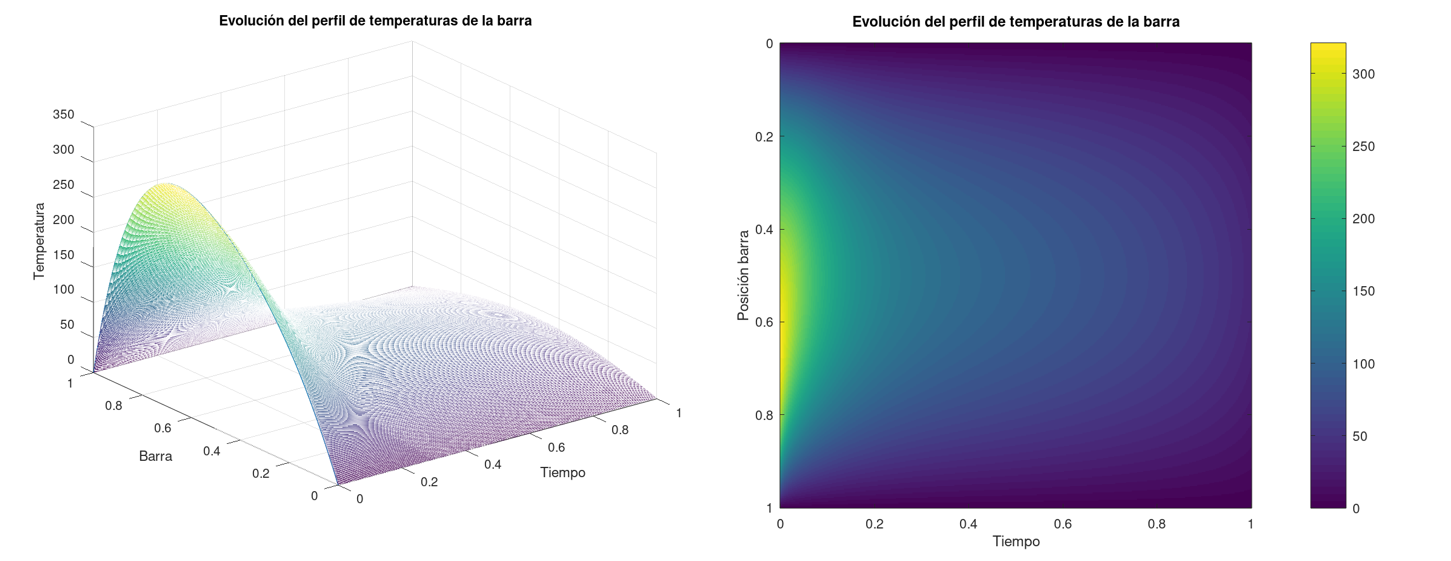
\includegraphics[scale=0.4]{sniplsode.PNG}
    \caption{Representación de los resultados del comando \textit{lsode} como \textit{heatmap} y gráfica-3D}
    \label{fig:lsodesnip}
\end{figure}
Simulando ahora con el $\theta$-método con los parámetros: $\theta=\{\frac{3}{4},\frac{1}{2}\},N=500,\Delta t = 2\times 10^{-3},K=500$. Se obtienen las siguientes representaciones:
\begin{figure}[H]
    \centering
    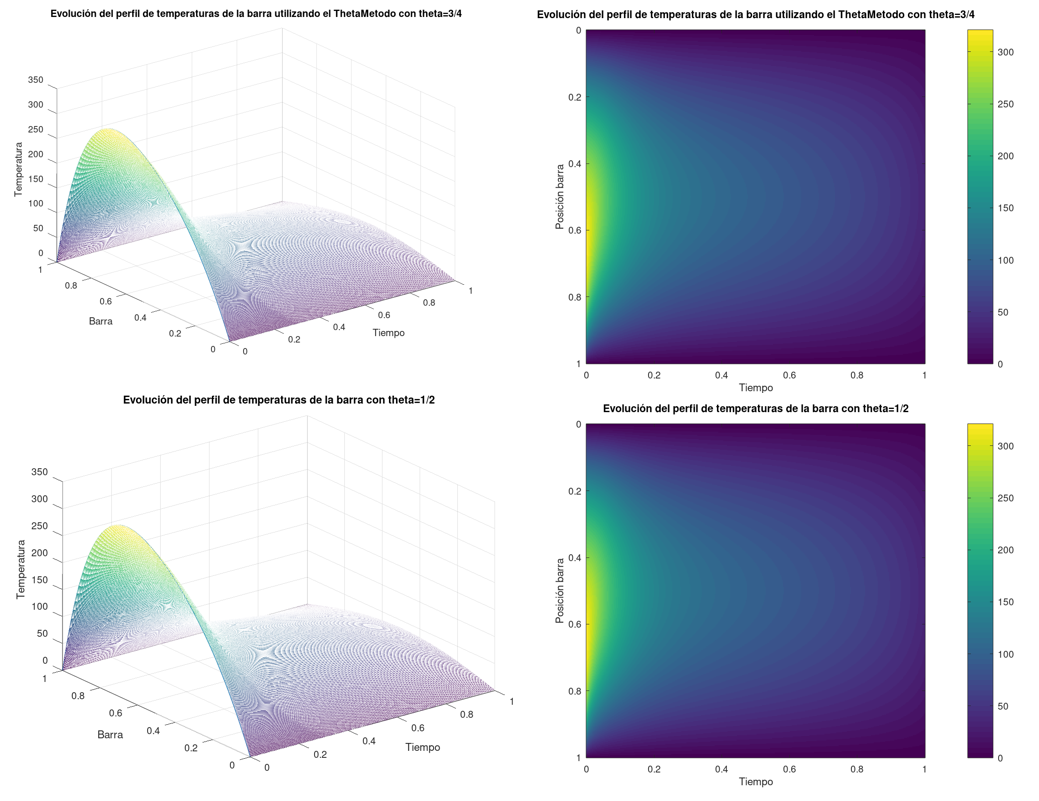
\includegraphics[scale=0.65]{megasnip.PNG}
    \caption{Representación de los resultados del $\theta$-método para $\theta=\frac{3}{4}$ (arriba) y $\theta=\frac{1}{2}$ (abajo) como \textit{heatmap} y gráfica-3D}
    \label{fig:megasnip}
\end{figure} 

Observamos que los resultados obtenidos (Fig \ref{fig:lsodesnip} y Fig. \ref{fig:megasnip}) son prácticamente iguales a simple vista. Para observar con más detalle la diferencia se construye un \textit{heatmap} adicional definido como el valor absoluto de la diferencia entre el $\theta$-método y \textit{lsode} en cada punto $(x_j,t^k)$:
\begin{figure}[H]
    \centering
    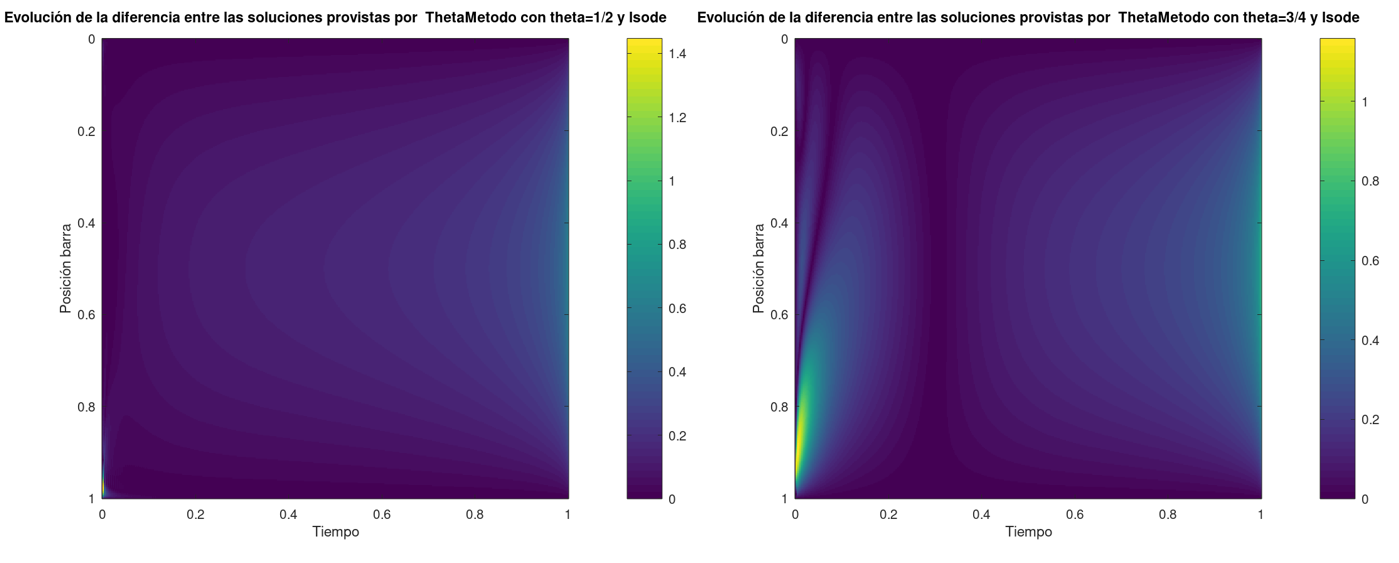
\includegraphics[scale=0.45]{diffsnip.PNG}
    \caption{Representación de la diferencia entre $\theta$-método con $\theta=\frac{3}{4}$ (derecha) y $\theta=\frac{1}{2}$ (izquierda) contra \textit{lsode} como \textit{heatmap}}
    \label{fig:comp75}
\end{figure}

Se aprecia un error de no más de una unidad para ambos valores de $\theta$ exceptuando un entorno particular en el tiempo alrededor de cero en la posición cercana a 1 para $\theta=\frac{3}{4}$. También se observa que el error es cada vez mayor cuanto más al centro de la barra se está y se va avanzando en $t$. Una posible interpretación es: dado que en los bordes por definición es $0 \ \forall \ t$, el error en los mismos es 0. Por lo que el error se amplificará al alejarnos de los bordes de la barra. Ya que la temperatura se calcula en base a ella misma y a su vecinos en el tiempo anterior (\ref{sistema_jj}). \

Por el otro lado, con $\theta=\frac{3}{4}$ se observa un comportamiento más errático. Recordando el diagrama \ref{fig:Diagrama} conjeturamos que $\theta=\frac{3}{4}$ aproxima la integral más acertadamente en ciertos puntos y en otros comete mayor error que el método del trapecio. De hecho, sabemos que la función $1000\sqrt{|1-t|}$ tiene derivada decreciente y la misma tiende a $-\infty$ a medida que nos acercamos al tiempo $t=1$. Por lo que, considerando el diagrama \ref{fig:Diagrama}, la recta entre dos puntos $(x_j,u(x_j))$ y $(x_{j+1},u(x_{j+1}))$ tendrá una pendiente negativa de considerable magnitud en $t\approx1$. Entonces la aproximación será peor cerca de este tiempo. Más aún, podemos notar que el error con $\theta=\frac{3}{4}$ es ligeramente mayor. Lo cual tiene sentido dado que se esta tomando como aproximación un trapecio que aproxima aún peor el área debajo de la gráfica. \

Considerando que el orden de la temperatura es de $10^2$, ambos métodos aproximan bastante bien a $u$ con los parámetros dados. Pero para este caso el método del trapecio lo hace mejor.

\subsection{Simulación del $\theta$-método con $f(x,t)=0$}
Esta situación, donde la barra se encuentra desprovista de una fuente calorífica, será también simulada utilizando
\textit{lsode} como referencia y el $\theta$-método con $\theta=0$ con el esquema \ref{theta00}. Se utilizan los
parámetros: $\theta=0,N=500,\Delta t = 2\times 10^{-3},K=500$. No obstante, \textbf{no} fue posible realizar la simulación del
$\theta$-método en estas condiciones. Esto era esperable ya que en este caso $\frac{h^2}{2\mu}=2\times10^{-6}$ por lo que no podemos asegurar la convergencia de la simulación debido a que la proposición \ref{asintprop} no se aplica. La siguiente imagen muestra el comportamiento de $u$ utilizando \textit{lsode}:
\begin{figure}[H]
    \centering
    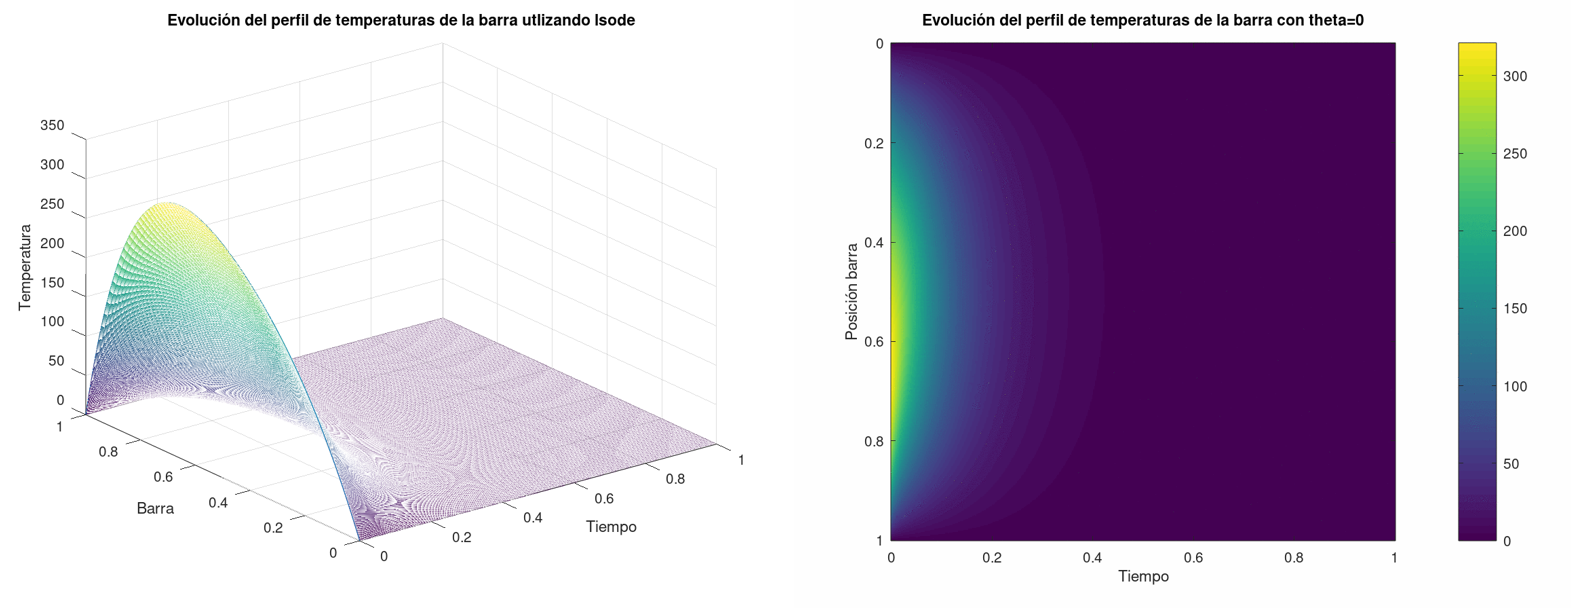
\includegraphics[scale=0.4]{snipf0.PNG}\label{fig:snipf0}
    \caption{Representación de los resultados del comando lsode con $f(x,t)=0$ mediante un \textit{heatmap} y gráfica-3D}
\end{figure}
Obsérvese que el calor global de la barra decrece más rápido con $f(x,t)=0$ que en el problema anterior con $f(x,t)=\sqrt{|1-t|}$. Esto tiene sentido dado que en el problema anterior se le estaba dando calor al sistema en cada instante $t$. Pero en este caso ya no se le esta proporcionando calor a la barra, y como la misma en sus 2 bordes tiene temperatura $0$ en todo $t$, la misma se va a estar enfriando hasta que la barra entera alcance temperatura nula.


\subsection{Error experimental del $\theta$-método}
En las condiciones del problema \ref{simusqrt}. Se estudia el error del  $\theta$-método comparándolo con la solución provista por el comando \textit{lsode}.
\begin{figure}[H]
    \centering
    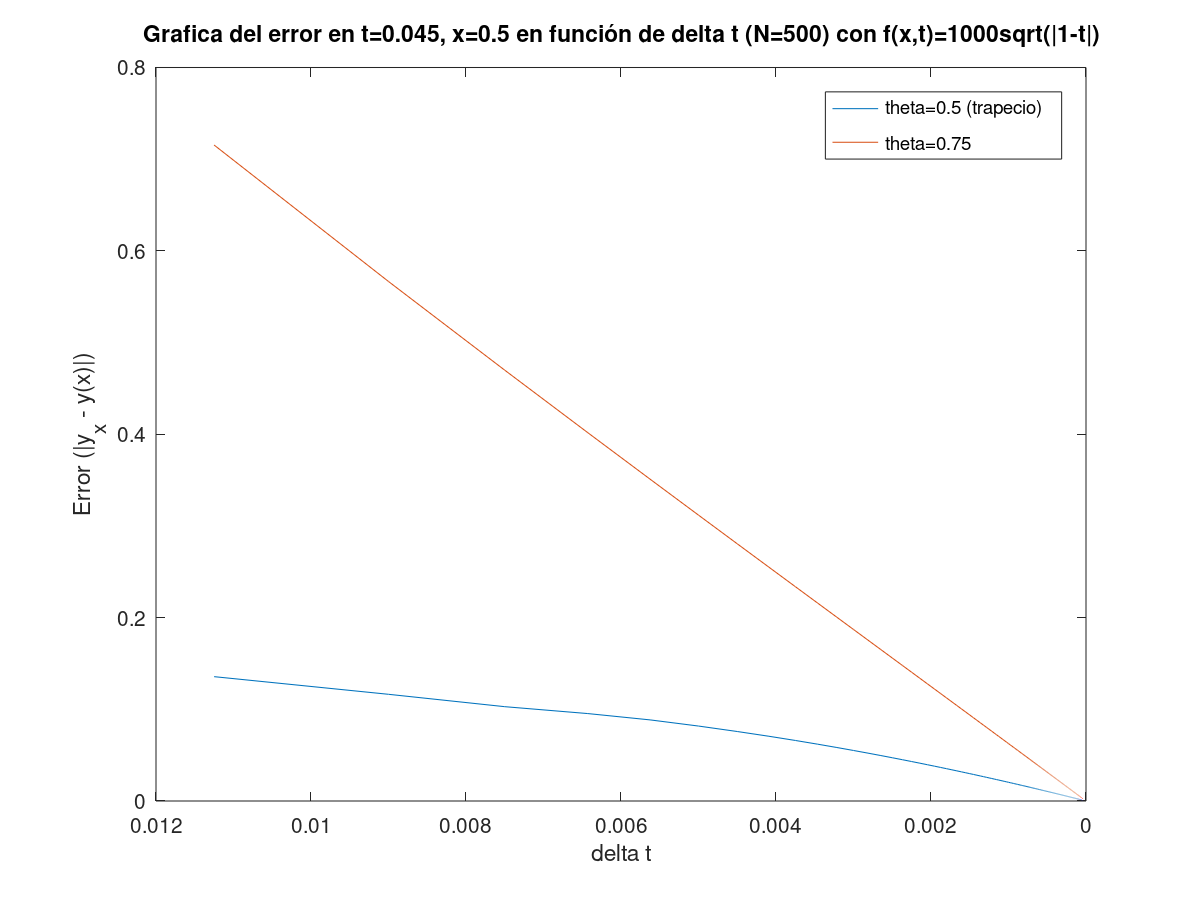
\includegraphics[scale=0.4]{errort50t75.png}
    \caption{Valor absoluto de la diferencia entre la solución provista por \textit{lsode} y el $\theta$-método en función de $\Delta t$.}
    \label{fig:snipf0}
\end{figure}
Podemos observar que el error de la aproximación cuando $\theta=\frac{1}{2}$ es menor que cuando $\theta=\frac{3}{4}$. Observar que el caso $\theta=\frac{1}{2}$ tiene un orden de decrecimiento mayor. Es decir, experimentalmente, el error del método del trapecio tiende a $0$ más rápido que el $\theta$-método con $\theta=\frac{3}{4}$. Estos resultados son acordes al orden analítico estudiado en la sección \ref{Errortheta}.\\
Por el otro lado, se estudia el error para el problema para el caso $f(x,t)=0$. Notar que para que el método tenga solución, necesitamos que $\Delta t < \frac{h^2}{2\mu}$:
\begin{figure}[H]
    \centering
    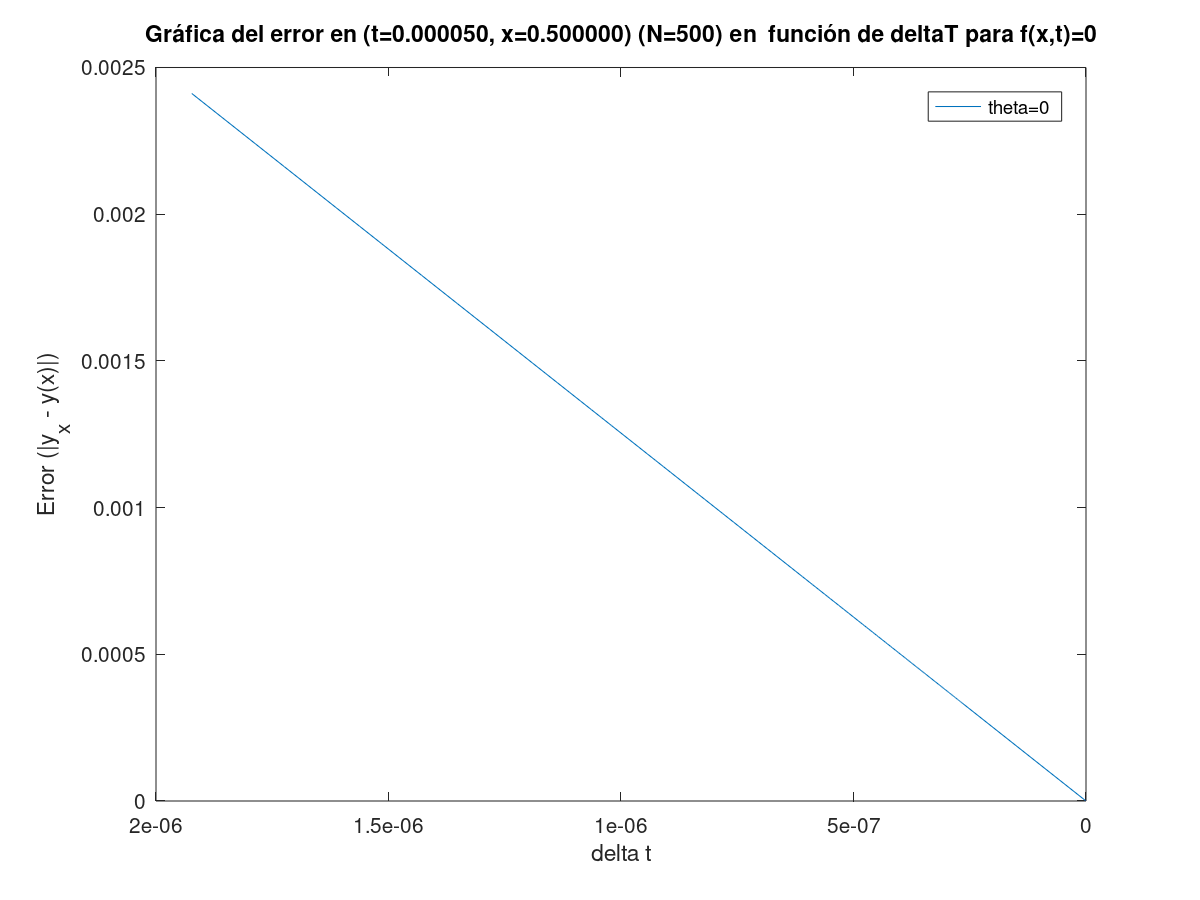
\includegraphics[scale=0.4]{e_t0.png}
    \caption{Valor absoluto de la diferencia entre la solución provista por \textit{lsode} y el $\theta$-método en función del $\Delta t$}
    \label{fig:snipf0}
\end{figure}
Se observa que la evolución del error con $\theta=0$ es similar a la de $\theta=\frac{3}{4}$. Lo cual es lo esperado dado que el orden del error del $\theta$-método es el mismo $\forall \ \theta \neq \frac{1}{2}$
\clearpage
\section{Conclusiones}\label{Conclusions}
Tras ahondar en la metodología que utiliza el $\theta$-método y confirmar experimentalmente su funcionamiento, hemos conseguido implementar el algoritmo y estudiar su comportamiento satisfactoriamente en las simulaciones planteadas. También demostramos un criterio de estabilidad asintótica para el caso particular $\theta=0, f(x,t)=0$. Concluimos que el $\theta$-método proporciona una aproximación satisfactoria de $u(x,t)$ con un error arbitrariamente pequeño definido por los parámetros $\Delta t, N$. También confirmamos experimentalmente que la evolución del error según $\Delta t$ es la esperada para los casos $\theta=\{0,\frac{1}{2},\frac{3}{4}\}$. Concluimos que para el problema planteado ($f(x,t)=1000\sqrt{|1-t|}$), el $\theta$-método con $\theta=\frac{1}{2}$ resulta superior.\\
Si bien las ecuaciones en derivadas parciales se utilizan para modelar una infinidad de fenómenos físicos, como es el caso de la evolución de la distribución del calor en una barra, resolverlas no es un problema sencillo. En la sección de metodología se realiza un extenso trabajo matemático para transformar este problema a uno de ecuaciones lineales. La demostración de la correctitud de los esquemas de resolución planteados para luego realizar su simulación es lo que consideramos como el logro principal de este informe.\\
Una futura linea de trabajo podría ser realizar pruebas experimentales más generales. Trabajando no solo en función de $\Delta t$ sino también en función de el tiempo y posición de la barra $(x,t)$. Aunque lo anterior puede traer dificultades debido al elevado tiempo de computo necesario para realizar las simulaciones.

%Tras un exhaustivo analisis podemos concluir que tanto por el theta metodo como por el metodo del trapecio se 
%puede llegar a una aproximación bastante buena de lo que buscabamos. Aunque como toda aproximación tiene un error cada método,
%pudimos ver que el error en el theta metodo es en un principio mucho mayor a el del metodo del trapecio, y va disminuyendo %considerablemente mas rapido que
%el del metodo del trapecio aproximandose ambos a 0 a medida que el Delta T se achica.  
%Cabe destacar que piccini se la come. :D
%\phantom{ piccini se la come. :D}
%\bibliographystyle{plain}

\bibliographystyle{endm.bst}
\bibliography{biblio}
\end{document}\grid


%TODO:
%   MEJORAR LAS GRAFICAS DE LOS ERRORES
%   REVISAR DETALLES
